%%%%%%%%%%%%%%%%%%%%%%%%%%%%%%%%%%%%%%%%%%%%%%%%%%%%%%%%%%%%%%%%%%%%%%%%%%%%%%%%%%%%%%%%%%%%%%%%%%%%%%%%%%%%%%%%%%%%%%%%%%%%%%%%%%%%%%%%%%%%%%%%%%%%%%%%%%%
% This is just an example/guide for you to refer to when submitting manuscripts to Frontiers, it is not mandatory to use Frontiers .cls files nor frontiers.tex  %
% This will only generate the Manuscript, the final article will be typeset by Frontiers after acceptance.
%                                              %
%                                                                                                                                                         %
% When submitting your files, remember to upload this *tex file, the pdf generated with it, the *bib file (if bibliography is not within the *tex) and all the figures.
%%%%%%%%%%%%%%%%%%%%%%%%%%%%%%%%%%%%%%%%%%%%%%%%%%%%%%%%%%%%%%%%%%%%%%%%%%%%%%%%%%%%%%%%%%%%%%%%%%%%%%%%%%%%%%%%%%%%%%%%%%%%%%%%%%%%%%%%%%%%%%%%%%%%%%%%%%%

%%% Version 3.4 Generated 2018/06/15 %%%
%%% You will need to have the following packages installed: datetime, fmtcount, etoolbox, fcprefix, which are normally inlcuded in WinEdt. %%%
%%% In http://www.ctan.org/ you can find the packages and how to install them, if necessary. %%%
%%%  NB logo1.jpg is required in the path in order to correctly compile front page header %%%

\documentclass[utf8]{frontiersSCNS} % for Science, Engineering and Humanities and Social Sciences articles
%\documentclass[utf8]{frontiersHLTH} % for Health articles
%\documentclass[utf8]{frontiersFPHY} % for Physics and Applied Mathematics and Statistics articles

%\setcitestyle{square} % for Physics and Applied Mathematics and Statistics articles
\usepackage{url,hyperref,lineno,microtype,subcaption}
\usepackage[onehalfspacing]{setspace}
\usepackage{booktabs}
\usepackage{amsmath}
\usepackage{amsfonts}
\usepackage{amssymb}
\usepackage{dsfont}
\usepackage{multirow}

\graphicspath{ {figures/} } %subfolder for images; set in preambel

%\linenumbers


% Leave a blank line between paragraphs instead of using \\


\def\keyFont{\fontsize{8}{11}\helveticabold}
\def\firstAuthorLast{Jäger {et~al.}} %use et al only if is more than 1 author
\def\Authors{Sebastian Jäger\,$^{1,*}$, Arndt Allhorn\,$^{1}$ and Felix Bießmann\,$^{1}$}
% Affiliations should be keyed to the author's name with superscript numbers and be listed as follows: Laboratory, Institute, Department, Organization, City, State abbreviation (USA, Canada, Australia), and Country (without detailed address information such as city zip codes or street names).
% If one of the authors has a change of address, list the new address below the correspondence details using a superscript symbol and use the same symbol to indicate the author in the author list.
\def\Address{$^{1}$Beuth University of Applied Sciences, Berlin, Germany}
% The Corresponding Author should be marked with an asterisk
% Provide the exact contact address (this time including street name and city zip code) and email of the corresponding author
\def\corrAuthor{Sebastian Jäger}
\def\corrEmail{sebastian.jaeger@beuth-hochschule.de}

\renewcommand{\vec}[1]{\mathbf{#1}}
\newcommand{\R}{\ensuremath{\mathds{R}}}

\newcommand{\code}[1]{\texttt{#1}}
\newcommand{\felix}[1]{\textcolor{red}{[Felix: #1]}}
\newcommand{\sebastian}[1]{\textcolor{blue}{[Sebastian: #1]}}
\newcommand{\arndt}[1]{\textcolor{green}{[Arndt: #1]}}


\begin{document}
\onecolumn
\firstpage{1}

\title[A Benchmark for Data Imputation Methods]{A Benchmark for Data Imputation Methods}

\author[\firstAuthorLast ]{\Authors} %This field will be automatically populated
\address{} %This field will be automatically populated
\correspondance{} %This field will be automatically populated

\extraAuth{}% If there are more than 1 corresponding author, comment this line and uncomment the next one.
%\extraAuth{corresponding Author2 \\ Laboratory X2, Institute X2, Department X2, Organization X2, Street X2, City X2 , State XX2 (only USA, Canada and Australia), Zip Code2, X2 Country X2, email2@uni2.edu}


\maketitle


\begin{abstract}
	%
	With the increasing importance and complexity of data pipelines, data quality became one of the key challenges in modern software applications. The importance of data quality has been recognized beyond the field of data engineering and database management systems (DBMS): Also, for machine learning (ML) applications, high data quality standards are crucial to ensure robust predictive performance and responsible usage of automated decision-making. One of the most frequent data quality problems is missing values. Incomplete data sets can break data pipelines and can have a devastating impact on downstream ML applications when not detected. While statisticians and, more recently, ML researchers have introduced a variety of approaches to impute missing values, comprehensive benchmarks comparing classical and modern imputation approaches under fair and realistic conditions are underrepresented. Here we aim to fill this gap. We conduct a comprehensive suite of experiments on a large number of data sets with heterogeneous data and realistic missingness conditions, comparing both novel deep learning approaches and classical ML imputation methods when either only test or train and test data are affected by missing data. Each imputation method is evaluated regarding the imputation quality and the impact imputation has on a downstream ML task. Our results provide valuable insights into the performance of a variety of imputation methods under realistic conditions. Further, they help to guide data preprocessing method selection for research as well as application.
	%
	\keyFont{ \section{Keywords:} data quality, data cleaning, imputation, missing data, benchmark, MCAR, MNAR, MAR} %All article types: you may provide up to 8 keywords; at least 5 are mandatory.
\end{abstract}


\section{Introduction}
\label{sec:introduction}

In recent years, complex data pipelines have become a central component of many software systems. It has been widely recognized that monitoring and improving data quality in these modern software applications is an important challenge at the intersection of database management systems (DBMS) and machine learning (ML) \citep{Schelter2015,Abedjan2018}. A substantial part of the engineering efforts required for maintaining large-scale production systems is dedicated to data quality, especially when ML components are involved \citep{Sculley2015,Bose2017b}.

Poor data quality can quickly break software applications and cause application downtimes, often leading to significant economic costs. Moreover, poor data quality can foster unfair automated decisions, which marginalize minorities or have other negative societal impacts~\citep{Stoyanovich2020,Yang2020,Bender2021}. For this reason, many researchers started investigating to what extent monitoring of data quality can be automated \citep{Abedjan2016,Baylor2017,Schelter2018,rukat2020towards}. While some aspects of such monitoring, like the consistency of data types, are easy to automate, others, like semantic correctness\footnote{A great example from life sciences is given in~\citep{Ziemann2016}}, are still the subject of active research~\citep{biessmann2021automated}. However, even if automatic monitoring tools, such as those proposed in~\cite{Schelter2017}, would be used, a central challenge remains: How can we automatically fix the detected data quality issues?

One of the most frequent data quality problems is \emph{missing values}~\citep{Kumar}. Reasons for incomplete data are manifold: data might be accidentally not recorded, lost through application or transmission errors, intentionally not filled in by users, or result from data integration errors.
%
Throughout the past decades, researchers from different communities have been contributing to an increasingly large arsenal of methods to impute missing values. Statisticians laid the theoretical foundations for missing value imputation \citep{Rubin} by describing different missingness patterns (more details in Section \ref{sec:missingess_pattern}). Statistical approaches have been proposed to handle missing values \citep{Graham}. Simple strategies include dropping incomplete observations or replacing missing values with constant mathematically valid values. While this might be a reasonable solution to ensure robust functioning of data pipelines, such approaches often reduce the amount of available data for downstream tasks and, depending on the missingness pattern, might also bias downstream applications~\citep{Stoyanovich2020,Yang2020} and thus further decrease data quality \citep{Little, Graham}. Other approaches popular in the statistics literature use more sophisticated modeling, such as multivariate imputation by chained equations (MICE)~\citep{Little,vanBuuren2018}.

More recently also ML approaches are increasingly used for imputation. Popular methods include k-nearest neighbors ($k$-NN)~\citep{Batista2003}, matrix factorization~\citep{Troyanskaya2001,Koren2009,Mazumder2010}, random forest-based approaches~\citep{Stekhoven2012}, discriminative deep learning methods~\citep{Biessmann2018a} as well as generative deep learning methods~\citep{GAIN, HIVAE, VAE_for_genomic_data, MisGAN, VIGAN}.

Most imputation studies provide solid experimental evidence that the respective proposed method in the application setting investigated outperforms other competitor's baselines. Yet, it remains hard to assess which imputation method consistently performs best in a large spectrum of application scenarios and data sets under realistic missingness conditions. In particular, most studies do not report both imputation quality and the impact of the imputation on downstream ML applications.

In this paper, we aim at filling this gap. We benchmark a representative set of imputation methods on a large number of data sets under realistic missingness conditions with respect to imputation quality and the impact on the predictive performance of downstream ML models. For our experiments, we use $69$ fully observed data sets from \code{OpenML} \citep{OpenML2013} with numeric and categorical columns. Each data set is associated with a downstream ML task (binary classification, multi-class classification, and regression). We run experiments by artificially introducing varying fractions of missing values of the three missingness patterns (MCAR, MAR, and MNAR, see also Section \ref{sec:methods}). We then measure both the imputation accuracy and impact on downstream performance in two application scenarios: (a) missing values in the test data, i.e., we train on complete data, and corrupt (and impute) only test data, and (b) both training and test data have missing values, i.e., we train and test on corrupted data.


The rest of this paper is structured as follows. In Section \ref{sec:related_work}, we review the related work on imputation benchmarking efforts and continue in Section \ref{sec:methods} with an overview of the missingness conditions and imputation methods investigated in this study. A detailed description of our benchmark suite and its implementation follows in Section \ref{sec:implementation}. The results of our experiments are described and visualized in Section \ref{sec:results}. We then highlight the key findings in Section \ref{sec:discussion} and, finally, draw our conclusions in Section \ref{sec:conclusion}.


\section{Related Work}
\label{sec:related_work}
%
The body of literature that is related to our work consists of two types of studies. Some focus on presenting new or improved imputation methods and compare them with existing and baseline approaches in broader settings, similar to benchmark papers \citep{Imputation_Benchmark_4, Imputation_Benchmark_6}. Others are benchmark studies and compare imputation strategies \citep{Imputation_Benchmark_1, Imputation_Benchmark_2, Imputation_Benchmark_3}. However, both have in common that they often focus on specific aspects or use cases and do not aim at an extensive comparison. In contrast, our goal is to get a broad overview of the following dimensions:
%
\begin{enumerate}
	\item Number and heterogeneity of data sets
	\item Varying downstream tasks (binary classification, multi-class classification, and regression)
	\item Realistic missingness patterns and amount of missing values
	\item Imputation methods and optimized hyperparameters
	\item Evaluation on imputation accuracy and impact on downstream task performance
	\item Training on complete and incomplete data
\end{enumerate}

\cite{Imputation_Benchmark_3} compared the downstream task performance on two binary classification data sets ($N = 48,842$, and $N = 435$) with imputed and incomplete data. Therefore, they varied the amount of MCAR and MNAR values from $0\%$ to $40\%$ in categorical features. For the imputation, they used six models: mode, random, $k$-NN, logistic regression, random forest, and SVM. The authors optimize the hyperparameters for one of the three downstream tasks but not for the imputation models. They conclude that using a $k$-NN imputation model performs best in most situations.

Similarly, \cite{Imputation_Benchmark_2} compare seven imputation methods (random, median, $k$-NN, predictive mean matching, Bayesian linear regression, linear regression, and non-bayesian) without optimizing their hyperparameters based on five small and numeric data sets (max. $1030$ observations). The authors discuss different missingness patterns but do not state which one they used in their experiments. However, they measured the methods' imputation performance for $10\%$ to $50\%$ missing values. Again, the authors show that $k$-NN imputation is best independent from the data set and missingness fraction.

\cite{Imputation_Benchmark_1} evaluate and compare seven imputation methods (random, mean, softImpute, miss-Forest, VIM kknn, VIM hotdeck, and MICE) combined with five classification models regarding their predictive performance. Therefore,  they use $13$ binary classification data sets with missing values in at least one column, which is why they do not know the data's missingness pattern. The amount of missing values ranges between $1\%$ and about $33\%$. In contrast to \cite{Imputation_Benchmark_3, Imputation_Benchmark_2}, the authors can cope with the situation where only incomplete data is available for training. In their setting, they could not find a single best imputation method. However, they show that the combination of imputation method, downstream model, and metric ($F1$ or $AUC$) influences the results.

The following two papers differ from others because they aim to compare their proposed method against existing approaches. \cite{Imputation_Benchmark_6} implement an iterative expectation-maximization (EM) algorithm that learns and optimizes a latent representation of the data distribution, parameterized by a deep neural network, to perform the imputation. They use ten classification and three regression task data sets and 11 imputation baselines (zero, mean, median, MICE, miss-Forest, softImpute, $k$-NN, PCA, autoencoder, denoising autoencoder, residual autoencoder) for comparison. The authors conducted both evaluations, imputation and downstream task performance, with $25\%$, $50\%$, and $75\%$ MNAR missing values and showed that their method outperforms the baselines.

To the best of our knowledge \citep{Imputation_Benchmark_4} is the largest and most extensive comparison, although the authors focus on introducing an imputation algorithm and present its improvements. Their proposed algorithm cross-validates the choice of the best imputation method out of $k$-NN, SVM, or tree-based imputation methods, where the hyperparameters are cross-validated, too. The authors then benchmarked their approach on $84$ classification and regression tasks against five imputation methods: mean, predictive mean matching, Bayesian PCA, $k$-NN, and iterative $k$-NN. They measured the imputation and downstream task performance on $10\%$ to $50\%$ MCAR and MNAR missing values. The authors show that their proposed method outperforms the baselines, closely followed by $k$-NN and iterative $k$-NN.

We summarize the mentioned papers and related benchmarks in Table \ref{tab:related_work}. Most benchmarks use broad missingness fractions but lack realistic missingness conditions or a large number of heterogeneous data sets. Further, no paper systematically compares the imputation quality and impact on downstream tasks for imputation methods trained on complete and incomplete data. Studies presenting novel imputation methods based on deep learning often lack a comprehensive comparison with classical methods under realistic conditions, with few exceptions~\citep{Imputation_Benchmark_6}. In contrast, we aim at a broad and comprehensive benchmark, which accounts for all dimensions mentioned in this section.

% Please add the following required packages to your document preamble:
% \usepackage{booktabs}
% \usepackage{multirow}
\begin{table}[]
	\centering
	\begin{tabular}{@{\extracolsep{4pt}}p{2cm}p{3cm}rp{1.5cm}p{1cm}llll@{}}
		\toprule
		\multicolumn{1}{c}{\multirow{2}{*}{Study}} & \multicolumn{1}{c}{\multirow{2}{*}{\# Data Sets/Tasks}} & \multicolumn{1}{c}{\multirow{2}{*}{\# B.}} & \multicolumn{2}{c}{Missingness}                             & \multicolumn{2}{c}{Evaluation}                       & \multicolumn{2}{c}{Training on}                         \\\cline{4-5} \cline{6-7}\cline{8-9}
		\\[-0.75em]
		\multicolumn{1}{c}{}                      & \multicolumn{1}{c}{}    & \multicolumn{1}{c}{}   & \multicolumn{1}{c}{Pattern} & \multicolumn{1}{c}{Fraction}                                    & \multicolumn{1}{c}{Imp.} & \multicolumn{1}{c}{Down.} & \multicolumn{1}{c}{Comp.} & \multicolumn{1}{c}{Incomp.} \\ \midrule
		\\[-.75em]
		\cite{Imputation_Benchmark_3}                                         & 2 binary clf.  & 6                                               & MCAR MAR                   & 0\% 10\% 20\% 30\% 40\%                                            & No                       & Yes                       & \multicolumn{2}{c}{\emph{unclear}}                             \\ \hline
		\\[-.75em]
		\cite{Imputation_Benchmark_2}                                         & 5 data sets      & 7                                          & \emph{unclear}                     & 10\% 20\% 30\% 40\% 50\%                                           & Yes                      & No                        & \multicolumn{2}{c}{\emph{unclear}}                         \\ \hline
		\\[-.75em]
		\cite{Imputation_Benchmark_1}                                         & 13 binary clf.    & 7                           & \emph{unclear*}                    & 1\% - $\sim$33\%                                                      & No                       & Yes                       & No                        & Yes                         \\\hline
		\\[-.75em]
		\cite{Imputation_Benchmark_6}                                         & 10 clf.\newline 3~~~regression     & 11                                  & MNAR                        & 25\% 50\% 75\%                                                       & Yes                      & Yes                       & \multicolumn{2}{c}{\emph{unclear}}                         \\\hline
		\\[-.75em]
		\citep{Imputation_Benchmark_4}                                         & 84 data sets\newline \footnotesize(clf. and regression)     & 5                                        & MCAR MNAR                  & 10\% 20\% 30\% 40\% 50\%                                           & Yes                      & Yes                       & \multicolumn{2}{c}{\emph{unclear}}                         \\\hline
		\\[-.75em]
		Ours                                      & 21 regression\newline 31 binary clf.\newline 17 multi-class clf.    & 6                 & MCAR MAR MNAR             & 1\% 10\% 30\% 50\%                                                  & Yes                      & Yes                       & Yes                       & Yes                         \\ \bottomrule
		\multicolumn{9}{l}{\footnotesize*Authors use incomplete datasets and, therefore, do not know the missingness pattern}
	\end{tabular}
	\caption{An overview of related benchmarks. In contrast to our benchmark, all other studies focus on specific aspects such as downstream tasks or missingness conditions. Most importantly, no paper systematically compares imputation methods trained on complete and incomplete data sets. Abbreviations: the symbol \emph{\#} stands for the number of, \emph{B.} means Baselines, \emph{Imp.} means Imputation Quality, \emph{Down.} means Impact on Downstream Task, \emph{Comp.} means Complete Data, \emph{Incomp.} means Incomplete Data, and \emph{clf.} means classification.}
	\label{tab:related_work}
\end{table}


\section{Methods}
\label{sec:methods}
%
One of the main goals of this work is to provide a comprehensive evaluation of missing value imputation methods under realistic conditions. In particular, we focus on two aspects: (a) a broad suite of real-world data sets and tasks and (b) realistic missingness patterns. The following sections describe the data sets and missingness patterns we considered and the data preprocessing steps. Then follows a detailed description of the compared imputation methods, the used hyperparameter optimization strategies, and metrics for evaluation.

\subsection{Data sets}
\label{sec:datasets}
%
We focus on a comprehensive evaluation with several numeric data sets and tasks (regression, binary classification, and multi-class classification). The OpenML database~\citep{OpenML2013} contains thousands of data sets and provides an API. The Python package \code{scikit-learn} \citep{scikit-learn} can use this API to download data sets and create well-formatted \code{DataFrames} that encode the data properly.

We filter available data sets as follows. To calculate the imputation performance, we need ground truth data sets without missing values. Moreover, especially deep learning models need sufficient data to learn their task properly. However, because we plan to run many experiments, the data sets must not be too big to keep training times feasible. For this reason, we choose data sets without missing values that contain 5 to 25 features and 3.000 to 100.000 observations. We then removed duplicated, corrupted, and Sparse ARFF\footnote{Attribute-Relation File Format} formatted data sets.

The resulting 69 data sets are composed of 21 regression, 31 binary classification, and 17 multi-class classification data sets. The supplementary material contains a detailed list of all data sets and further information, such as OpenML ID, name, and the number of observations and features.


\subsection{Missingness Patterns}
\label{sec:missingess_pattern}
Most research on missing value imputation considers three different types of missingness patterns:
%
\begin{itemize}
	\item Missing completely at random (MCAR, see Table \ref{tab:missingness_patterns_MCAR}): \\
	Values are discarded independently of any other values
	\item Missing at random (MAR, see Table \ref{tab:missingness_patterns_MAR}): \\
	Values in column $c$ are discarded dependent on values in another column $k\neq c$
	\item Missing not at random (MNAR, see Table \ref{tab:missingness_patterns_MNAR}): \\
	Values in column $c$ are discarded dependent on their value in $c$
\end{itemize}
%
The missingness pattern most often used in the literature on missing value imputation is MCAR. Here the missing values are chosen independently at random. Usually, the implementations of this condition draw a random number from an uniform distribution and discard a value if that random number was below the desired missingness ratio. Few studies report results on the more challenging conditions MAR and MNAR. We here aim for realistic modeling of these missingness patterns inspired by observations in large-scale real-world data sets as investigated in \cite{Biessmann2018a}. We use an implementation proposed in \cite{Schelter2020a} and \cite{Jenga}, which selects two random percentiles of the values in a column, one for the lower and one for the upper bound of the value range considered. In the MAR condition, we discard values if values in a random other column fall in that percentile. In the MNAR condition, we discard values in a column if the values themselves fall in that random percentile range.
%
\begin{table}
	\centering
	%	\caption{
	%		Examples of missingness patterns for a missingness ratio of 50\%. 	}
	%	\label{tab:missingness_patterns}
	%	\vspace{1em}
	%	\begin{subtable}{0.3\textwidth}
	\begin{minipage}{0.28\textwidth}
		\centering
		\begin{tabular}{cc}
			\toprule
			height &  height$_{\text{MCAR}}$ \\
			\midrule
			179.0 &                     ? \\
			192.0 &                     ? \\
			189.0 &                 189.0 \\
			156.0 &                 156.0 \\
			175.0 &                     ? \\
			170.0 &                 170.0 \\
			181.0 &                     ? \\
			197.0 &                     ? \\
			156.0 &                 156.0 \\
			160.0 &                 160.0 \\
			\bottomrule
		\end{tabular}
		\caption{
			Applying the MCAR condition to column \textit{height} discards five out of ten values independent of the height values.
		}
		\label{tab:missingness_patterns_MCAR}
		\vspace{2em}
	\end{minipage}
	\hfill
	\begin{minipage}{0.3\textwidth}
		\centering
		\begin{tabular}{ccc}
			\toprule
			height & gender &  height$_{\text{MAR}}$ \\
			\midrule
			200.0 &      m &                    ? \\
			191.0 &      m &                    ? \\
			198.0 &      f &                198.0 \\
			155.0 &      m &                    ? \\
			206.0 &      m &                    ? \\
			152.0 &      f &                152.0 \\
			175.0 &      f &                175.0 \\
			159.0 &      m &                    ? \\
			153.0 &      f &                153.0 \\
			209.0 &      m &                209.0 \\
			\bottomrule
		\end{tabular}
		\caption{In the MAR condition, \textit{height} values are discarded dependent on values in another column,  here \textit{gender}. All discarded \textit{height} values correspond to rows in which \textit{gender} was \textit{male}.
		}
		\label{tab:missingness_patterns_MAR}
	\end{minipage}
	\hfill
	\begin{minipage}{0.28\textwidth}
		\centering
		\begin{tabular}{cc}
			\toprule
			height &  height$_{\text{MNAR}}$ \\
			\midrule
			154.0 &                     ? \\
			181.0 &                 181.0 \\
			207.0 &                 207.0 \\
			194.0 &                 194.0 \\
			153.0 &                     ? \\
			156.0 &                     ? \\
			198.0 &                 198.0 \\
			185.0 &                 185.0 \\
			155.0 &                     ? \\
			164.0 &                     ? \\
			\bottomrule
		\end{tabular}
		\caption{In the MNAR condition, \textit{height} values are discarded dependent on the actual \textit{height} values. All discarded values correspond to small \textit{height} values.
		}
		\label{tab:missingness_patterns_MNAR}
		\vspace{1em}
	\end{minipage}

\end{table}

\subsection{Data Preprocessing}
\label{sec:preprocessing}
%
Data preprocessing is often an essential part of ML pipelines to achieve good results \citep{Sculley2015}. In our experiments, we apply the following three preprocessing steps for all imputation methods:
%
\begin{itemize}
	\item Encode categorical columns: \\
	Categories are transformed into a numerical representation, which is defined on the training set and equally applied to the test set

	\item Replace missing values: \\
	To avoid the imputation model from failing

	\item Normalize the data: \\
	Columns are rescaled to the same range, which is defined on the training set and equally applied to the test set
\end{itemize}
%
However, the concrete techniques for discriminative imputation, described in Sections \ref{sec:simple_imputation} to \ref{sec:dl_imputation}, and generative approaches, described in Section \ref{sec:generative_imputation}, are different.

For discriminative imputation approaches, we substitute missing values with their column-wise mean/mode value, one-hot encode categorical columns and normalize the data to zero mean and unit variance.
For generative imputation approaches, we need to preserve the number of columns. For this reason, we encode the categories of categorical columns as values from $0$ to $n-1$, where $n$ is the number of categories. Then, missing values are replaced with random uniform noise from $0$ to $0.01$, and, finally, the data is min-max scaled ranging from $0$ to $1$.

\subsection{Imputation Methods}
\label{sec:methods:impuation}
%
In this section, we describe our six different imputation methods. The overall goal of an imputation method is to train a model on a data set $\vec{X}\in\R^{n\times d} = [\vec{x}_1, \vec{x}_2, ..., \vec{x}_{i-1}, \vec{x}_{i+1}, ..., \vec{x}_d]$, where $d$ is the number of features, $n$ the number of observations, and $\vec{x}_i$ denotes the to-be-imputed column.
To abstract crucial steps such as preprocessing the data (see Section \ref{sec:preprocessing}) and cross-validating the imputation method's hyperparameters (see Section \ref{sec:HPO}), we define a framework implemented by all of the following imputation approaches.


\subsubsection{Mean/Mode Imputation}
\label{sec:simple_imputation}
%
As a simple imputation baseline, we use the column-wise \code{mean} for numerical or \code{mode}, i.e., the most frequent value,  for categorical columns to fill missing values.


\subsubsection{$k$-NN Imputation}
\label{sec:knKNN}
%
A popular ML imputation baseline is $k$-NN imputation, also known as Hot-Deck imputation~\citep{Batista2003}. For our implementation thereof, we use \code{scikit-learn}'s \code{KNeighborsClassifier} for categorical to-be-imputed columns and \code{KNeighborsRegressor} for numerical columns, respectively.


\subsubsection{Random Forest Imputation}
%
Similarly to the $k$-NN imputation approach, described in Section \ref{sec:knKNN}, we implement the random forest imputation method using \code{scikit-learn}'s \code{RandomForestClassifier}, and \code{RandomForestRegressor}.



\subsubsection{Discriminative Deep Learning Imputation}
\label{sec:dl_imputation}
%
Often simple deep learning models can achieve good imputation results~\citep{Biessmann2018a}. To easily optimize the model's architecture, we use the AutoML\footnote{"automated machine learning (AutoML) [...] automatically set [the model's] hyperparameters to optimize performance" \cite{AutoML}} library \code{autokeras} \citep{AutoKeras} to implement the discriminative deep learning imputation method.
For categorical columns, we use \code{autokeras}' \code{StructuredDataClassifier} and for numerical columns \code{StructuredDataRegressor}. Both classes take care of properly encoding the data themselves and optimizing the model's architecture and hyperparameters. We use $max\_trials = 50$, which means \code{autokeras} tries up to $50$ different model architecture and hyperparameter combinations, and $epochs = 50$, such that each model is trained for a maximum of $50$ epochs (\code{autokeras} uses early stopping by default).


\subsubsection{Generative Deep Learning Imputation}
\label{sec:generative_imputation}
%
All of the above approaches essentially follow the ideas known in the statistics literature as {\em fully conditional specification} (FCS) \citep{vanBuuren2018}: a discriminative model is trained on all but one column as features and the remaining column as the target variable. A well-known FCS method is multiple imputation with chained equations (MICE) \citep{Little}. FCS has the advantage to be applicable to any supervised learning method, but it has the decisive disadvantage that for each to-be-imputed column, a new model has to be trained. Generative approaches are different in that they train just one model for an entire table. All matrix factorization-based approaches, such as \cite{Troyanskaya2001,Koren2009,Mazumder2010}, can be thought of as examples of generative models for imputation. We do not consider those linear generative models here as they have been shown to be outperformed by the mentioned methods and focus on deep learning variants of generative models only.

Generative deep learning methods can be broadly categorized into two classes: (variational) autoencoders (VAE)~\citep{VAE}\footnote{We focus on probabilistic autoencoders here as there are more imputation methods available for VAEs} and generative adversarial networks (GAN)~\citep{GAN}. In the following, we shortly highlight some representative imputation methods based on either of these two and describe the implementation used in our experiments.

\paragraph{Variational Autoencoder (VAE) Imputation}
%
VAEs learn to encode their input into a distribution over the latent space and decode by sampling from this distribution \citep{VAE}. Imputation methods based on this type of generative model include \cite{HIVAE, VAE_for_genomic_data, VAEM}. Rather than comparing all existing implementations, we focus on the original VAE imputation method for the sake of comparability with other approaches. To find the best model architecture, i.e., the number of hidden layers and their sizes, we follow the approach proposed by \cite{CaminoVAE}. We optimized using zero, one, or two hidden layer(s) for the encoder and decoder and fixed their sizes relative to the input dimension, i.e., the table's number of columns. If existing, the encoder's first hidden layer has $50\%$ of the input layer's neurons and the second layer $30\%$. The decoder's sizes are vice versa for upsampling the information to the same size as the input data. The latent space is also fixed to $20\%$ of the input dimension.
For training, we use Adam optimizer with default hyperparameters, batch size of $64$, and early stopping within $50$ epochs.


\paragraph{Generative Adversarial Network (GAN) Imputation}
%
GANs consist of two parts - a generator and a discriminator \citep{GAN}. In an adversarial process, the generator learns to generate samples that are as close as possible to the data distribution, and the discriminator learns to distinguish whether an example is true or generated. Imputation approaches based on GANs include \cite{GAIN, VIGAN, MisGAN}.
Here we employ one of the most popular approaches of GAN-based imputation, Generative Adversarial Imputation Nets (GAIN)~\citep{GAIN}.
GAIN adapts the original GAN architecture as follows.
The generator's input is the concatenation of the input data and a binary matrix that represents the missing values. The discriminator learns to reconstruct the mask matrix. Its input is the concatenation of the generator's output and a hint matrix, which reveals partial information about the missingness of the original data. The computation of the hint matrix incorporates the introduced hyperparameter $hint\_rate$. A second hyperparameter GAIN introduces $\alpha$ helps to balance the generator's performance for observed and missing values.
For training, we use Adam optimizer with default hyperparameters except for the learning rate for generator and discriminator, batch size of $64$, and early stopping within $50$ epochs.


\subsection{Hyperparameter Optimization}
\label{sec:HPO}
%
Optimizing and cross-validating hyperparameters are crucial to gain insights into a models' performance, robustness, and training time. Therefore, we choose for each imputation model the, as we find, most important hyperparameters and optimize them using cross-validated grid-search. For the $k$-NN and random forest imputation methods, we use 5-fold cross-validation, whereas we only 3-fold cross-validate VAE and GAIN to reduce the overall training time. Table \ref{tab:HPO} gives an overview of all imputation approaches and their hyperparameters we optimize, and the number of combinations. We do not define hyperparameter grids for mean/mode and DL imputation, as the former is parameterless and the latter optimized by \code{autokeras}.
%
\begin{table}[]
	\centering
	\begin{tabular}{@{}llll@{}}
		\toprule
		\multirow{2}{*}{Imputation Method} & \multicolumn{2}{c}{Hyperparameters}                          & \multirow{2}{*}{Grid Size} \\\cline{2-3}
		\\[-0.75em]
		& \multicolumn{1}{c}{Name}        & \multicolumn{1}{c}{Values} &                            \\ \midrule
		Mean/Mode                         &                                 &                            &                           \\
		\\[-0.5em]
		$k$-NN                             & $n\_neighbors$                  & \{1, 3, 5\}                & 3                          \\
		\\[-0.5em]
		Random Forest                      & $n\_estimators$                 & \{10, 50, 100\}            & 3                          \\
		\\[-0.5em]
		Discriminative DL*                   &                                 &                            &                            \\
		\\[-0.5em]
		VAE                                & $n\_hidden\_layers$             & \{0, 1, 2\}                & 3                          \\
		\\[-0.5em]
		\multirow{4}{*}{GAIN}              & $alpha$                         & \{1, 10\}                  & \multirow{4}{*}{16}        \\
		& $hint\_rate$                    & \{0.7, 0.9\}               &                            \\
		& $generator\_learning\_rate$     & \{0.0001, 0.0005\}         &                            \\
		& $discriminator\_learning\_rate$ & \{0.00001, 0.00005\}       &                            \\ \bottomrule
		\multicolumn{4}{l}{\footnotesize*Optimized using \code{autokeras}, see Section \ref{sec:dl_imputation}}
	\end{tabular}
	\caption{An overview of all imputation methods and their hyperparameters we optimized. \emph{Mean/Mode} imputation does not have any hyperparameters, and \emph{Discriminative DL} is optimized using \code{autokeras}, which is why we do not explicitly define a hyperparameter grid.}
	\label{tab:HPO}
\end{table}



\subsection{Evaluation Metrics}
%
To evaluate our experiments, we use two metrics: root mean square error ($RMSE$) and $macro\ F1$-score.
%
The $RMSE$ is defined as:
%
\begin{equation}
	RMSE = \sqrt{\frac{1}{N} \sum_{i = 0}^{N} (y_i - \hat{y_i})^2}
	\label{eq:RMSE}
\end{equation}
%
where $N$ is the number of observations, $y_i$ the observed values, and $\hat{y}_{i}$ the predicted values.
The $macro\ F1$-score is defined as the mean of class-wise $F1$-scores:
%
\begin{equation}
	macro\ F1 = \frac{1}{C}\sum_{i = 0}^{C} F1_i
	\label{eq:F1}
\end{equation}
%
where $i$ is the class index, $C$ the number of classes and the definition of $F1$ is:
%
\begin{equation}
	F1 = \frac{TP}{TP + \frac{1}{2}(FP + FN)}
\end{equation}
%
where $TP$ is the number of true positives, $FP$ the number of false positives, and $FN$ the number of false negatives.

Imputing categorical columns can be seen as a classification task. Accordingly, we measure performance in this case and for downstream classification tasks by the $macro\ F1$-score. In the following, we use the terms $F1$-score and $F1$ synonymously for $macro\ F1$-score. For regression tasks and imputing numerical columns, we use the $RMSE$. Since $F1$ is a score measure, larger values imply better performance. On the other hand, $RMSE$ is an error measure: a smaller value indicates better performance.


\section{Implementation and Experiments}
\label{sec:implementation}
%
In this section, we describe our benchmark suite in detail and its implementation.

As described in Section \ref{sec:methods:impuation}, we define a framework that provides for each of the six implemented imputation approaches a common API with the methods \code{fit} and \code{transform}. \code{fit} trains the imputation model on given data while cross-validating a set of hyperparameters, and \code{transform} allows imputing missing values of the to-be-imputed column the imputation model is trained on. For our implementation, we use \code{tensorflow} version 2.4.1, \code{scikit-learn} version 0.24.1, and \code{autokeras} version 1.0.12.

The Python package \code{jenga}\footnote{Software package "to study the effects of common data corruptions (e.g., missing values, broken character encodings) on the prediction quality of ML models." Source: \url{https://github.com/schelterlabs/jenga}} \citep{Jenga} provides two features we use to implement our experiments. First, it implements the mechanisms to discard values for the missingness patterns MCAR, MAR, and MNAR, as described in Section \ref{sec:missingess_pattern}. Second, it provides a wrapper for OpenML data sets, creates an $80/20$ training-test split, and can automatically train a \emph{baseline model} for the downstream task defined by the data set. We use the default task settings of \code{jenga} in which \code{scikit-learn}'s \code{SGDClassifier}  is used for classification and \code{SGDRegressor} for regression tasks. As preprocessing steps, it first replaces missing values with a constant, and second, one-hot encodes categorical columns and normalizes numerical columns to zero mean and unit variance. Finally, to train a robust model, it 5-fold cross-validates the hyperparameters \emph{loss}, \emph{penalty}, and \emph{alpha} using grid search. \code{jenga} reports the baseline model's performance ($F1$ for classification, $RMSE$ for regression) on the test set.


\subsection{Experimental Settings}
%
Our experimental settings are listed in Table \ref{tab:experiment_settings}. Each experiment is executed three times, and the average performance metrics are reported.
%
\begin{table}
	\centering
	\begin{tabular}{ll}
		\toprule
		Parameter            & Values                                     \\ \midrule
		Data Sets             & 69 (see supplementary material)    \\
		\\[-0.5em]
		Imputation Methods              & Mean/Mode, $k$-NN, Random Forest, DL, GAIN, VAE \\
		\\[-0.5em]
		Missingness Patterns  & MCAR, MAR, MNAR                            \\
		\\[-0.5em]
		Missingness Fractions & $1\%, 10\%, 30\%, 50\%$                      \\ \bottomrule
	\end{tabular}
	\caption{Overview of our experimental settings. We focus on covering an extensive range of the dimensions described in Section \ref{sec:related_work}. In total, there are $4,968$ experiments, which we repeat three times to report the mean imputation/downstream score.}
	\label{tab:experiment_settings}
\end{table}
%
For each of the data sets, we sample one to-be-imputed column upfront, which remains static throughout our experiments.

We split the experiments into four parts. In \emph{Experiment 1}, we compare imputation approaches with respect to their imputation quality (Section \ref{sec:experiment_1}), and in \emph{Experiment 2}, we compare imputation methods with respect to the impact on downstream tasks (Section \ref{sec:experiment_2}). Both experiments are repeated in two application scenarios: \emph{Scenario 1} (with complete training data, see Section \ref{sec:scenario_1}) and \emph{Scenario 2} (with incomplete training data, see Section \ref{sec:scenario_2}).

\subsubsection{Experiment 1: Imputation Quality}
\label{sec:experiment_1}
%
With this experiment, we aim to reveal how accurately the imputation methods can impute the original values.
With the help of \code{jenga}, we spread the desired number of missing values across all columns of the test set. For a certain missingness pattern and fraction, e.g., $30\%$ MAR, we introduce $\frac{30\%}{N}$ missing values of this pattern to each of the $N$ columns.
The evaluation of the imputation quality is then performed using the to-be-imputed column's discarded values as ground truth and the imputation model's predictions. If the to-be-imputed column is categorical, we report the $F1$-score, and for numerical columns, the $RMSE$.


\subsubsection{Experiment 2: Impact on Downstream Task}
\label{sec:experiment_2}
%
In \emph{Experiment 2}, we evaluate the impact of the different imputation approaches on numerous downstream ML tasks. For discriminative models, it is necessary to train one imputation model for each column with missing values. This fact, combined with our large number of experimental conditions (see Table \ref{tab:experiment_settings}), results in vast computational costs. To reduce those, while covering all relevant experimental conditions, we decided to discard values only in the test sets' to-be-imputed column.

To summarize, the entire experimental procedure is as follows:
%
\begin{enumerate}
	\item We train the baseline model of the downstream ML task on the training set and report its $baseline$ score ($F1$ for classification and $RMSE$ for regression tasks) on the test set.
	\item After discarding values in the to-be-imputed column, we again use the trained baseline model and calculate its score on the incomplete test set, hence the name: $incomplete$.
	\item We then impute the missing values of the test set and, once more, using the trained baseline model, calculate the $imputed$ score.
	\item Finally, we report the impact on the downstream task's performance as the percent change of the imputation over the incomplete data relative to the baseline performance on fully observed test data:
\end{enumerate}
%
\begin{equation}
	impact\ on \ downstream\ task = \frac{imputed - incomplete}{baseline}
	\label{eq:impact}
\end{equation}
%



\subsubsection{Scenario 1: Training on Complete Data}
\label{sec:scenario_1}
%
ML researchers commonly use complete (or fully observed) data to train, tune, and validate their ML applications. This is a reasonable assumption as the quality of the training data can be controlled better than that of the test data when the model is deployed in production. For instance, one can use crowdsourced tasks to collect all necessary features in the training data or use sampling schemes that ensure complete and representative training data. In this scenario, one can easily train an imputation model on complete data and use it to impute missing values in the test data before it is fed into the downstream ML model. We use \emph{Scenario 1} to simulate such situations and run both experiments, as described in Section \ref{sec:experiment_1} and \ref{sec:experiment_2}.

\subsubsection{Scenario 2: Training on Incomplete}
\label{sec:scenario_2}
%
Another common scenario is that not only the test data but also the training data have missing values. Thus, the imputation and downstream ML model has to be trained on incomplete training data. Also, in this scenario, we should expect missing values in the test data, which have to be imputed before applying the downstream ML model. To evaluate this application scenario, we adapt \emph{Experiment 1} and \emph{Experiment 2} slightly.

We first introduce missing values in the training and test set and then train the baseline and imputation models based on these incomplete data. The calculation of the imputation quality (\emph{Experiment 1}, Section \ref{sec:experiment_1}) remains the same. However, to calculate the impact on the downstream task, we lack the availability of the $baseline$ score on complete data. Therefore, we adapt Equation \ref{eq:impact} by replacing the $baseline$ denominator with $incomplete$. That means, in this scenario, we report the percent change of the imputation over the incomplete data relative to the downstream task performance on incomplete data:
%
\begin{equation}
	impact\ on \ downstream\ task = \frac{imputed - incomplete}{incomplete}
	\label{eq:impact_scenario2}
\end{equation}
%


\section{Results}
\label{sec:results}

In this section, we describe and visualize the results of our experiments. For the visualization, we choose to use box plots for all four experiments/scenarios. These allow us to get a decent impression of the distribution of the results based on quantiles. In contrast, the confidence bands of line charts would overlap too much to derive meaningful interpretations.  The vertical split represents the increasing difficulty for the missingness patterns: MCAR, MAR, and MNAR. To show different effects of imputing categorical or numerical columns, we further split the plots horizontally.  Because we randomly sample on target column for each data set, there are about $13\%$ categorical ($9$) and $87\%$ numerical ($60$) columns. Respectively, for the second experiment, the horizontal split presents classification and regression downstream tasks, which are also imbalanced: $48$ classification ($\sim70\%$) and $21$ regression tasks ($\sim30\%$).


\subsection{Experiment 1: Imputation Quality}

In this experiment, we evaluate the imputation performance of each method when training on complete data. As described above, our goal was to provide a broad overview of the imputation methods' performance on various data sets. Using randomly sampled to-be-imputed columns on heterogeneous data leads to a wide range of values for their evaluation metric ($F1$/$RMSE$), making it difficult to compare. To solve this problem, we split the results into categorical and numerical imputations and compute the rank for each imputation method and missingness pattern and fraction combination separately. Since we use six imputation methods, there are six ranks, where rank one is best and rank six the worst. If two or more methods perform equally, we assign the same rank, and for methods that failed during training, rank six.



\subsubsection{Scenario 1: Training on Complete Data}
\label{sec:results_experiment1_scenario1}

\begin{figure}\centering
	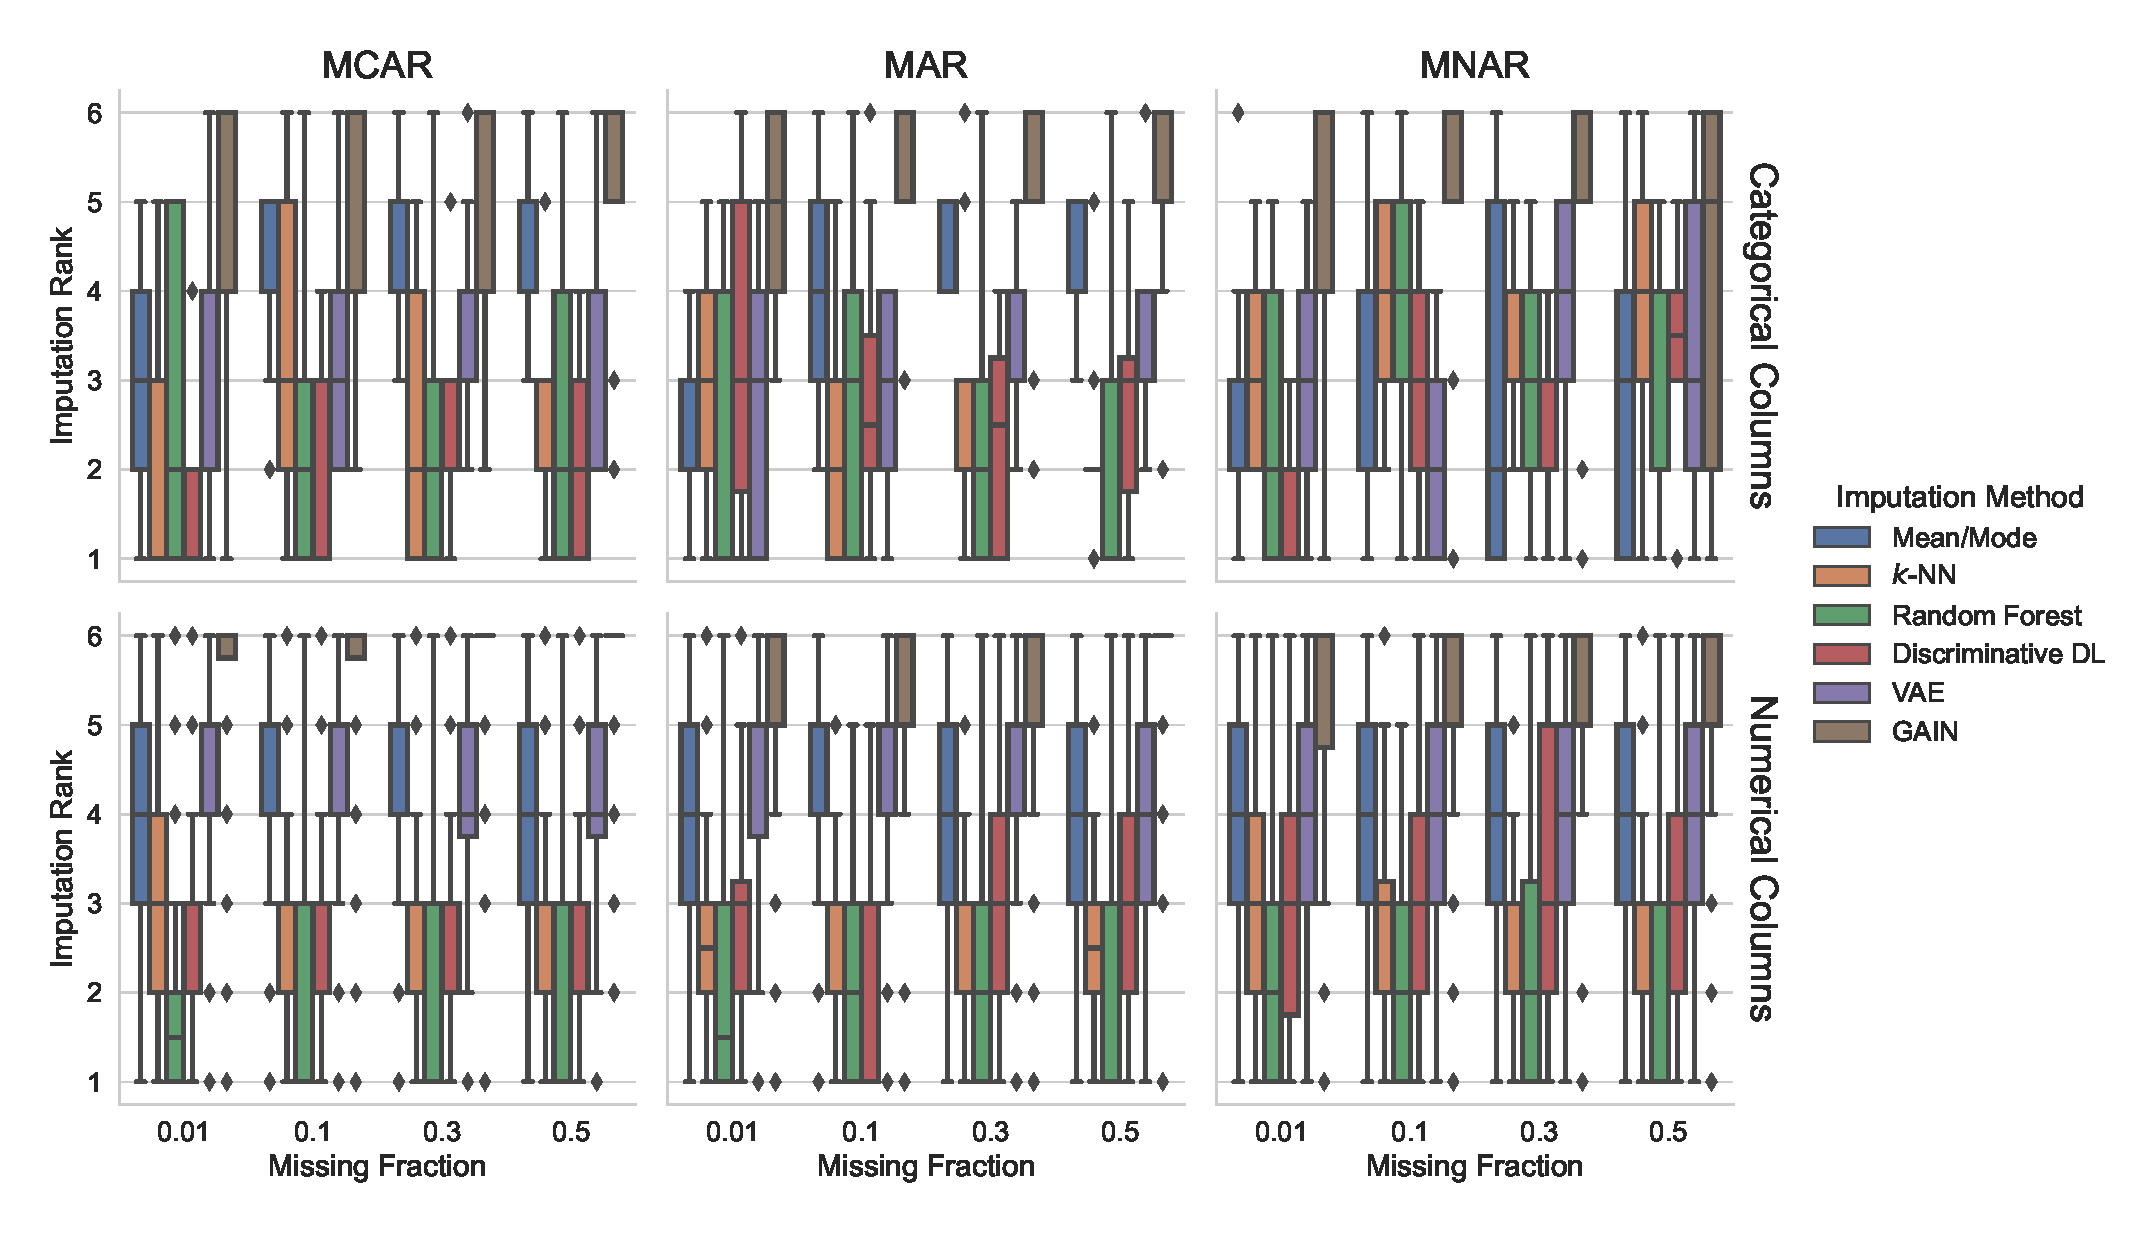
\includegraphics[width=1\columnwidth]{fully_observed_impute_rank_boxplot}
	\caption{Imputation ranks of the  imputation methods trained on complete data. Ranks are computed for each experimental condition characterized by data set, missingness pattern, and missingness ratio. In most conditions, random forest, $k$-NN, and discriminative DL perform best. Generative deep learning methods tend to perform worst. In the most challenging MNAR condition, mean/mode imputation achieves competitive results.
	}
	\label{fig:fully_observed_impute_rank_boxplot}
\end{figure}


Figure \ref{fig:fully_observed_impute_rank_boxplot} presents the imputation results when training on complete data. In about $33\%$ of these results, GAIN failed during training and got assigned the worst rank six.

When imputing categorical columns, there is no clear best method. However, in many settings, the discriminative DL approach achieves in $75\%$ of the cases at least rank three or better. Very similar but slightly worse results are shown by the random forest imputation method. For MCAR with $50\%$ missing values and MAR with $10\%$ to $50\%$ missingness, the $k$-NN imputation approach performs well and gets for $75\%$ of the cases at least rank three or better. VAE achieves in $50\%$ of the cases a rank between two and four. GAIN shows in most settings consistently the worst performance: rank four or worse in $75\%$ of the cases. Interestingly, mean/mode imputation scores better ranks for the more complex settings with MNAR missingness pattern.

When imputing numerical columns, the differences are more pronounced. Random forest is the only method that achieves one of the first three ranks in $75\%$ of the cases throughout all experimental conditions. Also, $k$-NN shows good results, ranking second or third in most settings in $50\%$ of the cases. Very similar results are achieved by the discriminative DL method that tends to lose performance from MAR with $30\%$ missingness to MNAR with $50\%$ missing values. Again VAE ranges most of the time between rank three and five, similar to mean/mode imputation, and GAIN gets the worst ranks five and six.

To summarize, simple imputation methods, such as $k$-NN and random forest, often perform best, closely followed by the discriminative DL approach. However, for imputing categorical columns with MNAR missing values, mean/mode imputation often performs well, especially for high fractions of missing values. The generative approaches get middle ranks (VAE) or range on the worst ranks (GAIN).

\subsubsection{Scenario 2: Training on Incomplete Data}


\begin{figure}\centering
	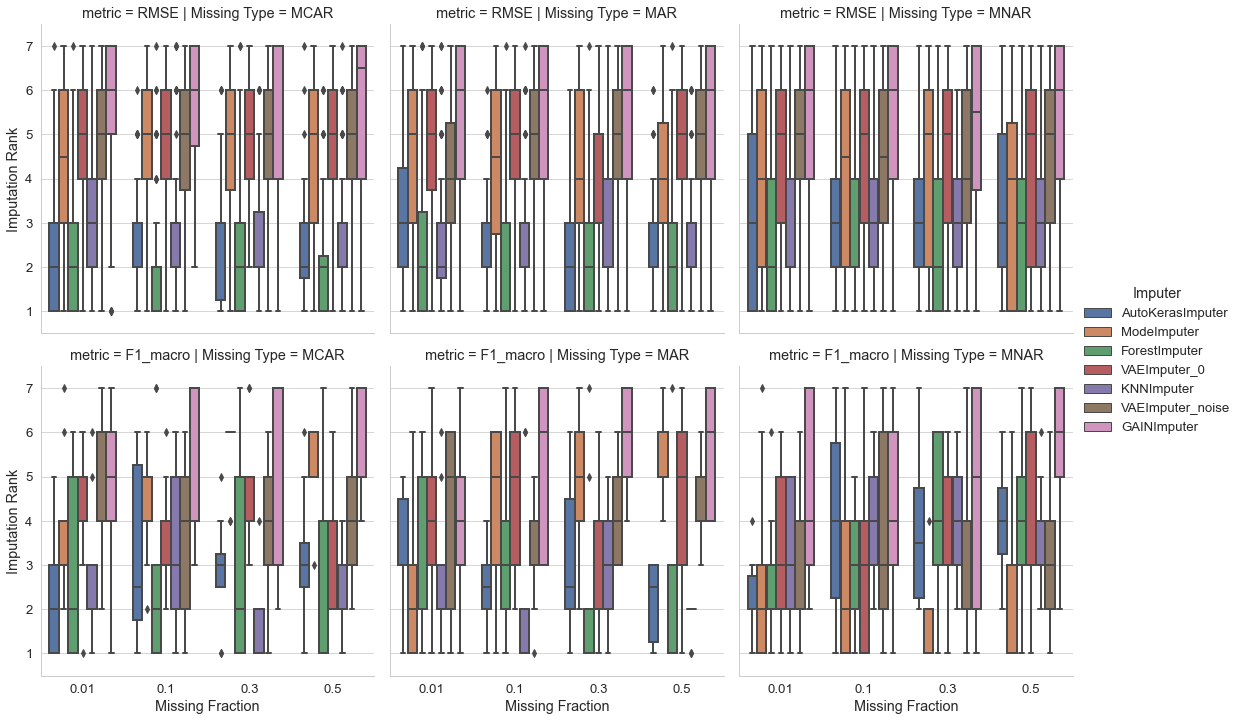
\includegraphics[width=1\columnwidth]{corrupted_impute_rank_boxplot}
	\caption{Imputation ranks of the  imputation methods trained on incomplete data. Ranks are computed for each experimental condition characterized by data set, missingness pattern, and missingness ratio. Similar to the training on fully observed data random forest, $k$-NN and discriminative DL perform better than generative deep learning methods in most settings. In the MNAR conditions, the imputation quality of all imputation approaches degrades in favor of mean/mode that outperforms the other for $30\%$ and $50\%$ missingness.}
	\label{fig:corrupted_impute_rank_boxplot}
\end{figure}

\autoref{fig:corrupted_impute_rank_boxplot} shows the imputation performance in \textit{Scenario 2}, i.e. when training on incomplete data. Imputing categorical columns with increasing difficulty, the ranks of mean/mode imputation improves. From MCAR $30\%$ to MNAR $50\%$, $k$-NN is in $75\%$ of the cases on at least the third rank or better, often it ranges on the first and second rank. For MNAR, its performance degrades gradually in favor of mean/mode that shows surprisingly good results, especially for the most challenging settings (MNAR with $30\%$ and $50\%$ missing values) where it outperforms others in at least $75\%$ of the cases. Random forest has very high variance, but on most missingness fractions with MCAR pattern, it ranks in $50\%$ of the cases on rank two or better. For MNAR, its rank improves with higher missingness fractions, whereas this trend reverses for MAR. In most cases, the generative methods rank worst (GAIN) and on the middle ranks (VAE). However, with high missingness and when missing values are MNAR, they can perform better.

Similar to the fully observed training case (Section \ref{sec:results_experiment1_scenario1}), imputation on numerical columns yields a clearer ranking than for categorical missing values. The imputation methods $k$-NN and random forest rank best with a tendency of random forest to outperform $k$-NN, where random forest's variance is higher. The discriminative DL approach yields a very similar performance to the $k$-NN for MCAR and MAR settings. In the more challenging MNAR setting, it ranks slightly worse. For MCAR, mean/mode imputation ranks in almost all settings in $50\%$ of the cases between rank four and five, for MAR and MNAR between rank three and five. Again the generative methods rank in almost all settings in $75\%$ of the cases worse than rank four, where VAE seldom ranks worst.

Overall, \textit{Scenario 1} (Figure \ref{fig:fully_observed_impute_rank_boxplot}) and \textit{Scenario 2} (Figure \ref{fig:corrupted_impute_rank_boxplot}) results for numerical columns are very similar. GAIN has become better in Scenario 2, although it still ranks worst. For categorical columns, generally, the ranks show higher variance. Most imputation methods worsen when the experimental settings' difficulty is higher, especially for MNAR, except for mean/mode, which ranks better for MNAR. This effect is even explicit when training on incomplete data. Generally, using methods, such as $k$-NN or random forest, achieves best results in most settings and cases.



\subsection{Experiment 2: Impact on Downstream Task}

In this experiment, we evaluate the imputation method's impact on the downstream performance in two scenarios: the imputation model was trained on complete and incomplete data. As described in Section \ref{sec:experiment_2}, this time, we discard only values in the data set's randomly sampled target column. We exclude the experiment setting, which failed during training the imputation model, i.e., there are about $33\%$ fewer results for the first scenario (training on complete data).


\subsubsection{Scenario 1: Training on Complete Data}

\begin{figure}\centering
	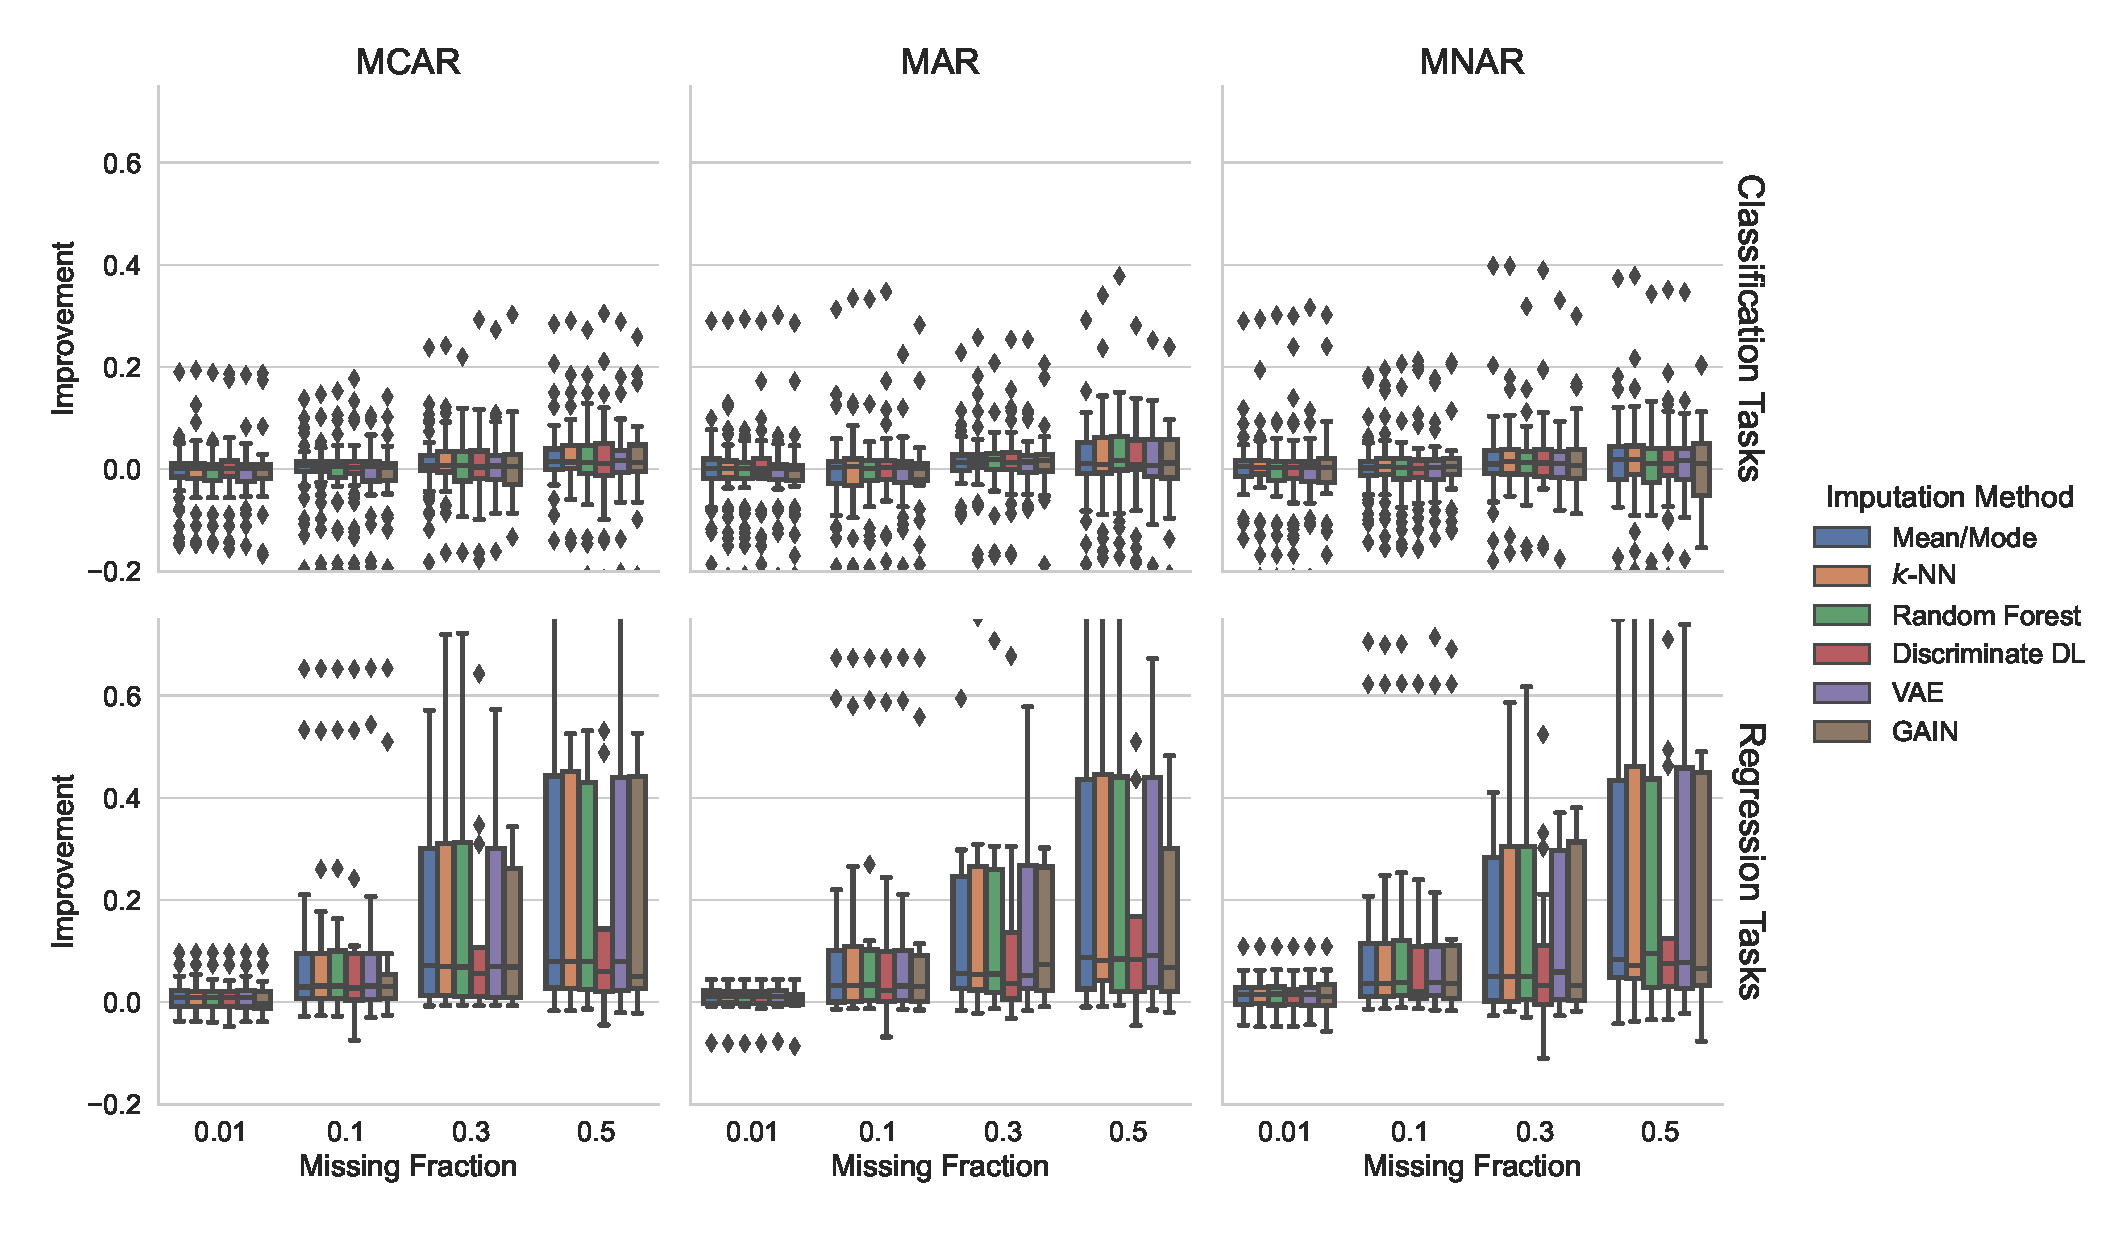
\includegraphics[width=1\columnwidth]{fully_observed_downstream_boxplot}
	\caption{Does imputation on incomplete test data improve predictive performance of a downstream ML model? We plot the improvement of the downstream ML model after imputation with imputation models trained on fully observed data. The downstream performance is compared to the performance obtained on incomplete test data, normalized by the ML model performance on fully observed test data. Overall, the classical ML methods and discriminative DL perform best achieving relative improvements of up to 10\% and more relative to fully observed test data.
	}
	\label{fig:fully_observed_downstream_boxplot}
\end{figure}

Figure \ref{fig:fully_observed_downstream_boxplot} visualizes how much the predictive performance of a downstream ML model improves compared to incomplete test data and normalized by the downstream performance obtained on fully observed test data (Equation \ref{eq:impact}). This metric is labeled \textit{Improvement} and represented on the plots' y-axis.

In all cases, using imputation approaches increase the downstream performance in $75\%$ of the cases. Not surprisingly, independent from the downstream task and the missingness pattern, the more missing values exist, the better the potential improvement, shown by the method's increasing median and $75\%$ quantile.

For regression tasks, all imputation methods on all settings degrade the performance in less than $25\%$ of the cases. Further, they hold great potential for improving the performance in the range of $\sim10\%$ and $\sim15\%$ for $30\%$ and $50\%$ MCAR or MAR missing values. However, there is a tendency from MCAR to MNAR that the potential performance degrades. In most settings, random forest's median improvement is best, followed by $k$-NN and discriminative DL. This effect also holds for their potential improvement ($75\%$ quantile), except for $50\%$ MNAR, where it is about five percentage points higher than the others. In most settings, VAE and mean/mode increase the downstream performance very similar but worse than the other three, and GAIN is always the worst.

For classification tasks, few imputation methods in some settings show degrading performance in slightly more than $25\%$ of the cases. However, their median imputation performance is always positive and generally higher than for regression tasks. In general, the potential improvements of the methods are in all settings roughly the same. As for regression tasks, random forest, followed by $k$-NN and discriminate DL, hold in $50\%$ of the cases the best performance. Unfortunately, this degrades from MCAR to MNAR. Surprisingly, this time GAIN holds much more potential improvement and performs in many settings better than VAE, especially when the missingness fraction is high.

All in all, independent from the experimental settings, random forest performs in $50\%$ of the cases best, closely followed by $k$-NN and discriminative DL. In general, when using imputation, the expected improvement is for classification higher than for regression tasks. This effect also holds for the missingness fractions: the higher the missingness fraction, the higher the potential improvements. Only in less than $25\%$ of all cases, we found degraded downstream performance.


\subsubsection{Scenario 2: Training on Incomplete Data}

\begin{figure}\centering
	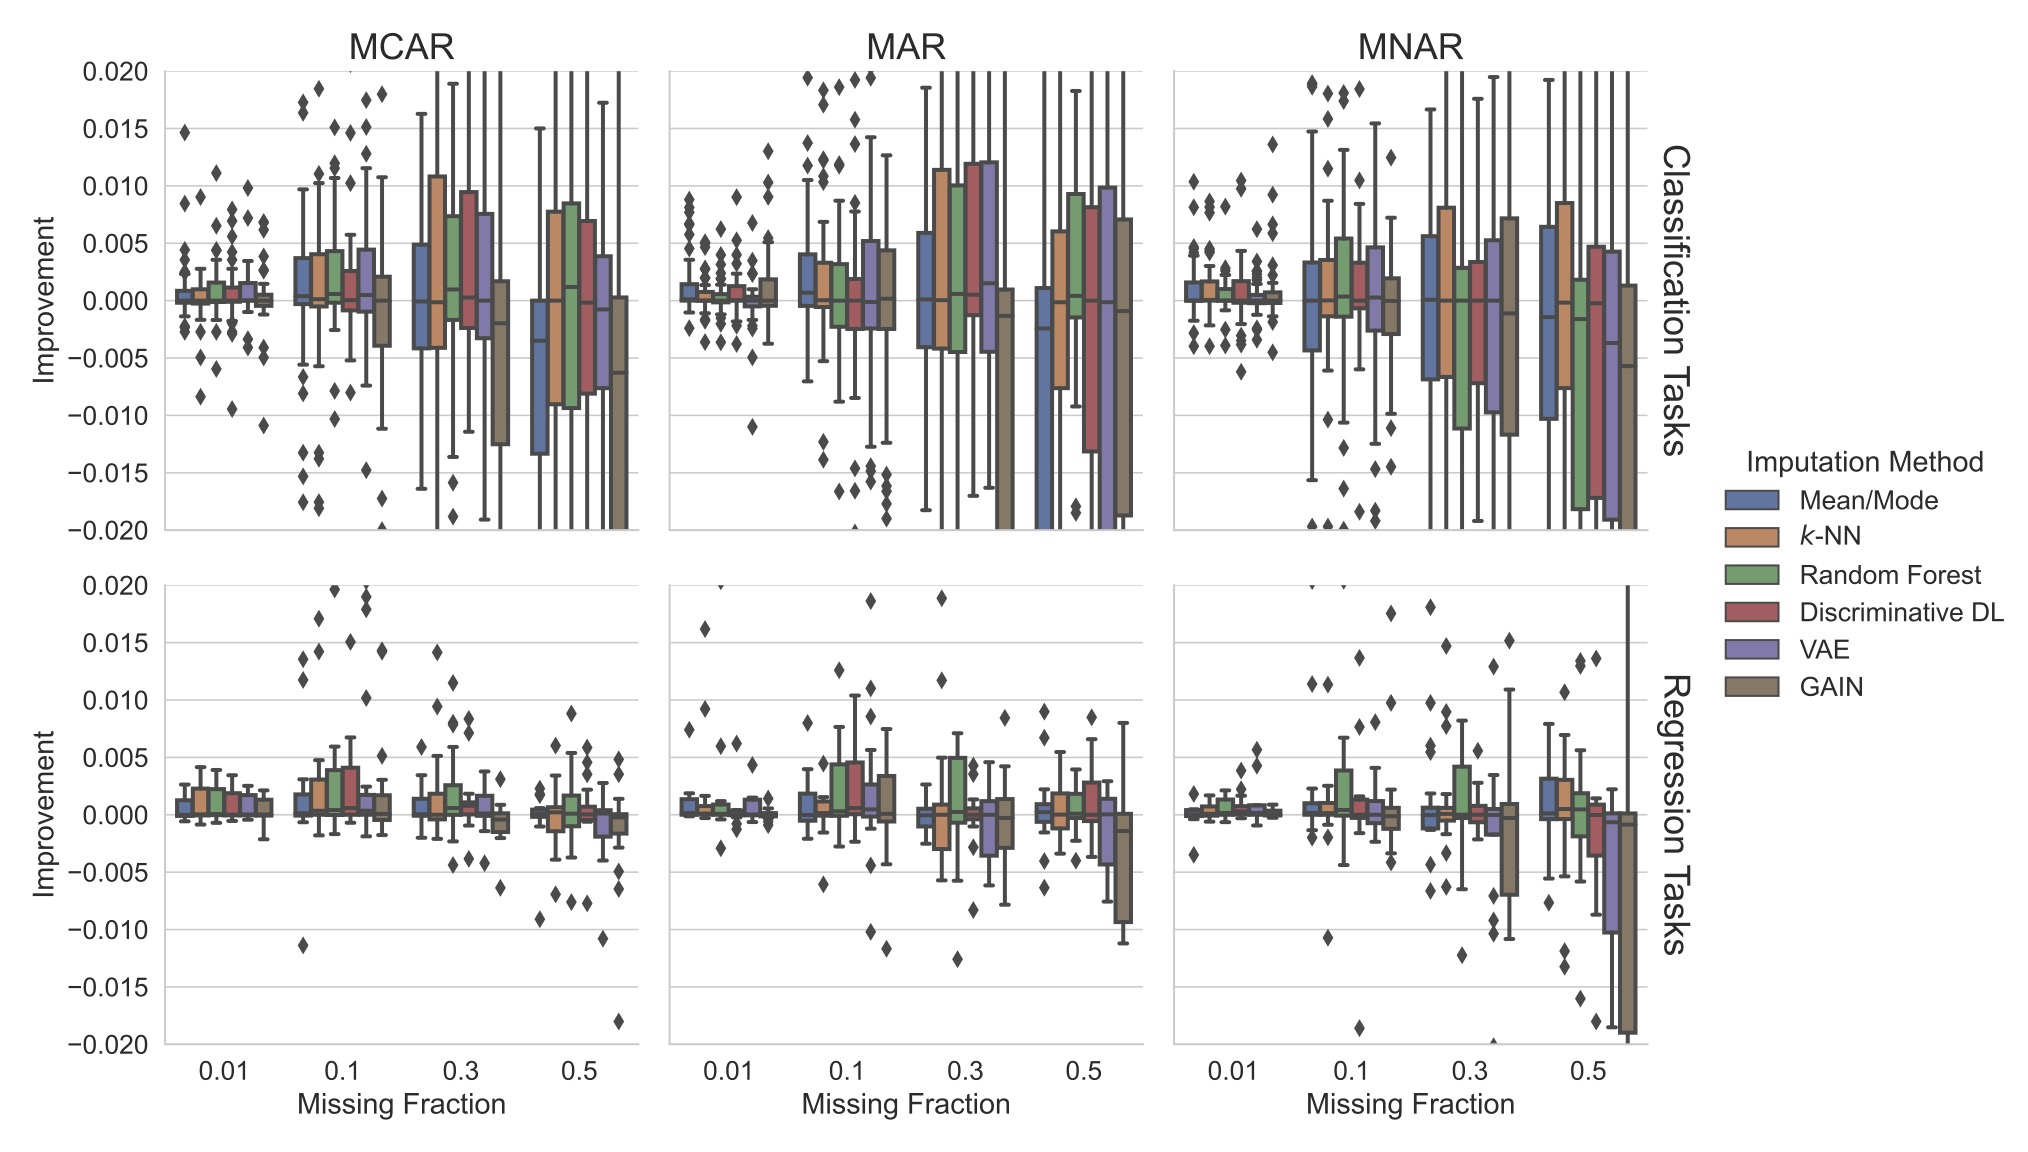
\includegraphics[width=1\columnwidth]{corrupted_downstream_boxplot}

	\caption{Impact on the downstream task of the six imputation methods trained on incomplete data. In regression tasks, no considerable improvements are achieved. In some cases, imputation worsened the downstream ML model. In classification tasks, in contrast, we observe slightly positive effects in some settings, but negative effects predominate in the harder settings.
	}
	\label{fig:corrupted_downstream_boxplot}
\end{figure}


Figure \ref{fig:corrupted_downstream_boxplot} illustrates the impact imputation has on the downstream task. We show how many percent the predictive performance of a downstream ML model improves compared to incomplete test data. This metric is labeled \textit{Improvement} and represented on the plots' y-axis. Here, the different scaling must be taken into account, i.e., the relative improvements are considerably smaller compared to the first scenario. One reason for this is the different basis for calculating the relative values (see Sections \ref{sec:experiment_2} and \ref{sec:scenario_2}).

The potential improvements when the imputation methods are trained on incomplete data are marginal. In all settings, there are hardly any improvements greater than $1\%$. However, with $30\%$ missing values or fewer, most cases have a positive impact.

For classification tasks, with up to $30\%$ MCAR or MAR missingness, there for all imputation methods, but GAIN, mostly very small but positive improvements, where higher missing fractions yield potentially higher improvements ($75\%$ quantile). However, high missingness fractions shift the improvements into the negative range, i.e., degrade the performance. For MNAR only for $1\%$ and $10\%$ missing values, we see mostly improvements, and for $30\%$ or $50\%$ missingness, the downstream performance degrades in most cases.

For regression tasks, there are hardly any potential improvements over $0.5\%$. On the other hand, there are also much fewer cases where imputation potentially degrades the performance. Outstanding is random forest, which yields in most settings the highest performance and the generative approaches that harm the performance when missingness is $30\%$ or higher.

To summarize, for up to $30\%$ missing values independent of the missingness pattern or downstream tasks, imputation increases the performance in most cases. Using random forest holds the best chance in almost all settings to improve the downstream performance.


\subsection{Computational Complexity}
%
Our results demonstrate that simple ML methods are often on par with modern deep learning methods. An important question in this context is how the various methods compare in terms of their computational complexity: if methods yield similar predictive performance, it is preferable to use those alternatives with the least computational effort. To measure the training and inference time, we use a sub-set of our experiments: all data sets, missingness fractions, and imputation methods (shown in Table \ref{tab:experiment_settings}) with MCAR pattern. We first train the imputation method on complete data, then discard values of the given missingness fraction in the training set, and impute those missing values. The wall-clock run time is measured in seconds when calling our framework's \code{fit} and \code{transform} methods (see Section \ref{sec:implementation} for details), which means that the training duration incorporates hyperparameter optimization (see Section \ref{sec:HPO} for details).

Because training and inference time depends heavily on the data set's size, directly averaging all experiments for the imputation methods leads to very similar mean but extremely high standard deviation values. For this reason, we first compute the mean duration and the standard deviation relative to its mean separately for training and inference for the imputation methods on each data set. Second, we average those values for each imputation method and present them in Table \ref{tab:time}. Using this approach helps to average overall experiments and, at the same time, gives indicators for the training and inference durations, as well as their variance.
%
\begin{table}
	\centering
	\begin{tabular}{@{\extracolsep{4pt}}lrrrr@{}}
		\toprule
		\multirow{2}{*}{Imputation Method} & \multicolumn{2}{c}{Training} & \multicolumn{2}{c}{Inference} \\\cline{2-3}\cline{4-5}
		\\[-0.75em]
		& Mean Duration &   Rel. SD & Mean Duration &   Rel. SD \\
		\midrule
		Mean/Mode &      0.005 &  0.550 &      0.029 &  0.171 \\
		\\[-0.5em]
		$k$-NN &     41.204 &  0.254 &       7.018 &  0.602 \\
		\\[-0.5em]
		Random Forest &    226.077 &  0.119 &     24.048 &  0.236 \\
		\\[-0.5em]
		Discriminative DL &   6275.019 &   0.405 &    440.389 &  0.211 \\
		\\[-0.5em]
		VAE &     71.095 &  0.099 &      11.215 &  0.085 \\
		\\[-0.5em]
		GAIN &    878.058 &  0.312 &     137.966 &  0.083 \\
		\bottomrule
	\end{tabular}
	\caption{Training and inference duration for each imputation method in seconds. We use the wall-clock run time to measure the durations for training, including hyperparameter optimization and inference for all data sets with MCAR missingness pattern and all fractions shown in Table \ref{tab:experiment_settings}. Because training and inference durations depend heavily on the data set size, we first calculate the durations' mean and relative standard deviation for each imputation method on every data set. Second, we average those mean durations and relative standard deviations for the imputation methods and present them as \emph{Mean Duration} and \emph{Rel. SD} separately for \emph{Training} and \emph{Inference}. Abbreviations: \emph{Rel. SD} means Relative Standard Deviation.
	}
	\label{tab:time}
\end{table}

As expected, if the imputation model's complexity increases, their training duration increases too, most of the time by multiple factors. There are two exceptions: discriminative DL and VAE, an explanation for this could be their number of hyperparameter combinations optimized during training. VAE optimizes only three, GAIN $16$ and discriminative DL $50$ combinations, representing their training durations order.

Similarly, the inference time increases with the model's complexity. The differences are clear but not as high as for the training durations.
Higher inference standard deviations, e.g., for $k$-NN and random forest (and discriminative DL), indicate that the best hyperparameters found strongly vary with the experimental settings and influence the model's computational complexity for inference. One reason for the discriminative DL's and GAIN's high training standard deviations could be the usage of early-stopping and, at the same time, indicate that it is important to try a huge number of hyperparameters to achieve good results. For mean/mode, the high standard deviation is likely an artifact of the very small training duration. Changes in milliseconds for computations are common and represent a large change relative to the mean/mode imputation's mean duration.

To summarize, the increasing complexity of the imputation methods is represented in their training and inference duration. For training more complex models, this is supported by a higher variance of training time, indicating the necessity to try a wide range of hyperparameters. On the other hand, once found, the hyperparameters for generative models influence the inference time less than for $k$-NN or random forest, whose prediction times depend heavily on the hyperparameters.


\section{Discussion}
\label{sec:discussion}

We investigated the performance of classical and modern imputation approaches on a large number of heterogeneous data sets under realistic conditions. In the following, we highlight some of the key findings.

\subsection{Simpler Imputation Methods Yield Competitive Results}
%
When evaluating imputation quality, our results demonstrate that simple supervised learning methods achieve competitive results, and in many cases, outperform modern generative deep learning-based approaches. In particular, in the MCAR and MAR setting, we see in Figures \ref{fig:fully_observed_impute_rank_boxplot} and \ref{fig:corrupted_impute_rank_boxplot} that $k$-NN, random forest, and the discriminative DL approach are, for at least $50\%$ of the cases, among the better ranks one, two, or three. Random forest tends to achieve the best rank more often. This effect is largely independent of whether the imputation methods are trained on complete or incomplete data.

This finding is in line with \cite{Imputation_Benchmark_3, Imputation_Benchmark_2, Imputation_Benchmark_4}. In these previous studies, the authors report that $k$-NN imputation is the best choice in most situations. However, \cite{Imputation_Benchmark_2, Imputation_Benchmark_4} did not incorporate a random forest imputation method. Other comparisons show a slight advantage of discriminative deep learning methods over random forests \citep{biessmann2019datawig}, but these experiments were conducted on a much smaller selection of data sets.

For categorical columns (see Figure \ref{fig:fully_observed_impute_rank_boxplot} and \ref{fig:corrupted_impute_rank_boxplot}, upper row) in the more challenging imputation settings MAR or MNAR with large missingness fractions, the mean/mode imputation tends to achieve better ranks. This effect can be attributed to the fact that the sets of observed categorical values often have small cardinality. Especially for skewed distributions, using the most frequent value to substitute missing values is a good approximation of the ground truth. If the training data contains a large fraction of missing values, the underlying dependencies exploited by learning algorithms are difficult to capture. For this reason, mean/mode scores for higher MNAR missing values in $75\%$ of the cases on rank two or better (visualized in Figure \ref{fig:corrupted_impute_rank_boxplot}). \cite{Imputation_Benchmark_3} did not explicitly calculate the ranks but their plots show the same tendency.

Since GAIN failed in about $33\%$ of settings when training data was complete, this could be a reason why, in most cases, GAIN achieves the worst ranks (see Figure \ref{fig:fully_observed_impute_rank_boxplot}). This is supported by the fact that GAIN does not fail for settings with incomplete training data, and often shows better ranks (see Figure \ref{fig:corrupted_impute_rank_boxplot}).

All in all, using random forest, discriminate DL, or $k$-NN are good choices in most experimental settings and promise the best imputation quality. However, incorporating the model's training and inference time, presented in Table \ref{tab:time}, shows that the discriminative DL approach is substantially slower for training and inference than the other two methods. This is because we used the expensive default model optimization of AutoKeras. Exploring fewer hyperparameters could decrease its imputation performance drastically. The training duration's high variance indicates that trying a large number of hyperparameters is necessary for good performance because early stopping would finish the training if the model converges. $k$-NN's standard deviation for inference is in contrast to random forest very high. This is expected as the inference time grows exponentially with the number of training data points. We conclude that given the similar performance of $k$-NN and random forests when the training data set is large, random forests (or similar methods) should be preferred over naive $k$-NN implementations. Alternatively, one might use appropriate speedups for the nearest neighbor search, such as $kd$-trees or approximate nearest neighbor search.

To summarize, the best performing imputation approach is random forest. It not only ranks best in most experimental settings, but it also shows a good balance of training, including optimizing hyperparameters and inference time that is not influenced by the training set size. However, when coping with data sets that miss $30\%$ or more values of the pattern MNAR, imputing categorical columns with their mode is very often the best choice.


\subsection{Substantial Downstream Improvements when Imputation Method was Trained on Complete Data}
%
Our results show that imputation can have a substantial positive impact on predictive performance in downstream ML tasks. We observe improvements in the downstream task of 10\% to 20\% in more than 75\% of our experiments. This holds for most imputation methods; we did not observe a clear advantage for an imputation method overall. Taking into account the considerable differences in wall-clock run time, our results indicate that also when choosing an imputation method that is both fast and improves downstream predictive performance random forests would be the preferred imputation method.

The positive impact of imputation on downstream performance is most pronounced when the imputation methods were trained on fully observed data. When imputation methods were trained on incomplete data, the positive impact of imputing missing values in the test data was substantially lower, sometimes even negative. While this might seem a disadvantage we emphasize that in many application use cases we can ensure that the training data be fully observed, for instance by acquiring more data before training the imputation as well as the downstream ML model.


\subsection{Limitations}
\label{sec:limitations}
%
Because one of the main goals of this study is a comprehensive comparison of imputation methods on a large number of data sets and missingness conditions, we made some decisions that limit our results.

Firstly, the used data sets consist of a maximum of $25$ features and $100k$ observations. For this reason, we can not conclude from our experiments how the imputation methods perform on large-scale data sets. Further, our data sets only contain numerical or categorical columns and no image- or text-based data, e.g., used in other deep learning-based imputation approaches \citep{Biessmann2018a}. However, in that work, the authors only considered text data as an input field to an imputation method, not as a column that could be imputed. Generally, most modern ML applications that involve text data are based on rather sophisticated natural language models. Combinations of such models with tabular data are an important field of research \citep{Yin2020} but beyond the scope of most imputation research so far.

Secondly, to measure the imputation impact on the downstream performance, we discarded and imputed values in only a single column. Therefore, the impact depends heavily on the chosen column's importance (e.g., see \cite{Jenga}). Generally, the impact when using an imputation model could vary when multiple columns are affected by missing values.



\section{Conclusions}
\label{sec:conclusion}
%
To the best of our knowledge, this is the first benchmark that compares classical and modern imputation approaches on a large number of datasets under realistic missingness conditions with respect to the imputation quality and the impact on the predictive performance of a downstream ML model. We also evaluated how the results changed when the imputation and downstream model were trained on incomplete data.

Our results can be summarized in two main findings. First, we demonstrate that imputation helps to increase the downstream predictive performance substantially regardless of the missingness conditions. When training data is fully observed, improvements for classification tasks were in more than 75\% of the cases between $10\%$ and $20\%$ and for regression tasks around $15\%$.

Second, we find that in almost all experiments, random forest-based imputation achieves the best imputation quality, and consequently also on the most data sets the best improvements on the downstream predictive performance. This finding is in line with previous imputation benchmark research in more constrained experimental conditions see also Section \ref{sec:related_work}. Yet, some aspects of these results appear at odds with some recent work on deep learning methods. While we are aware of the limitations of our experiments, see also Section \ref{sec:limitations}, we still argue that to better assess the value of most deep learning methods, it is helpful to stress test these methods under realistic conditions in large unified benchmarks with heterogeneous data sets \citep{Sculley2018, Bender2021}.






\bibliographystyle{frontiersinSCNS_ENG_HUMS} % for Science, Engineering and Humanities and Social Sciences articles, for Humanities and Social Sciences articles please include page numbers in the in-text citations
%\bibliographystyle{frontiersinHLTH&FPHY} % for Health, Physics and Mathematics articles
\bibliography{data-imputation}

%%% Make sure to upload the bib file along with the tex file and PDF


\end{document}
